\documentclass[11pt,a4paper]{article}

\usepackage[T1]{fontenc}
\usepackage[utf8]{inputenc}
\usepackage[margin=1in]{geometry}
\usepackage{amsmath,amssymb,amsthm,mathtools}
\usepackage{tikz}
\usetikzlibrary{positioning,arrows.meta,decorations.pathmorphing,calc,fit,
                backgrounds,graphs,graphs.standard,quotes}
\usepackage{pgfplots}
\pgfplotsset{compat=1.18}
\usepackage{xcolor}
\usepackage{booktabs}
\usepackage{array}
\usepackage{microtype}
\usepackage{hyperref}

\hypersetup{colorlinks=true,linkcolor=blue,citecolor=blue,urlcolor=blue}
\definecolor{stable}{HTML}{1B7837}
\definecolor{unstable}{HTML}{C2272D}
\definecolor{neutralg}{HTML}{4D4D4D}
\definecolor{accent}{HTML}{2166AC}
\definecolor{accent2}{HTML}{B2182B}
\definecolor{fieldc}{HTML}{D9730D}

\theoremstyle{plain}
\newtheorem{proposition}{Proposition}
\newtheorem{remark}{Remark}

\newcommand{\R}{\mathbb{R}}
\newcommand{\E}{\mathbb{E}}

\title{The Mediating Field\\[3pt]
\large A substrate-independent account of collective attention:\\
bioelectric gradients, pheromone trails, neural mean-fields,\\
and social norms are one mechanism}
\author{Internal note --- IWAI 2026 paper}
\date{2026-05-20}

\begin{document}
\maketitle

\begin{abstract}
Three turns of literature review converged on a single picture, and this
note records it. The way a collection of agents ``listens'' to one another
need not be a pairwise aggregation rule that we design by hand. Across
wildly different substrates --- Levin's bioelectric morphogenetic fields,
Deneubourg's pheromone trails, the mean-field of a neural population, and
the shared norms of a scientific community --- nature uses \emph{the same
motif}: a slow, shared field sits ``in the middle,'' every agent deposits
into it and reads out of it, and \emph{reading the field is what attention
to the collective \emph{is}}. Pairwise opinion pooling is the special,
degenerate case in which each agent privately recomputes the field every
step. Promoting the field to a first-class, shared, slowly-relaxing object
with its own (possibly nonlinear) dynamics (i)~makes ``trust'' a property
of how an agent reads the field rather than a decorative reweighting,
(ii)~resolves the decentralisation problem of a community-level prior
(the field \emph{is} the externalised prior, \`a la stigmergy), and
(iii)~relocates the bistability we have been chasing to where it belongs:
the self-consistency between fast agents and the slow field.
\end{abstract}

\section{The motif: couple through a field, not pairwise}
\label{sec:motif}

Our current substrate couples agents pairwise. Each agent~$i$ relaxes toward
the trust-weighted opinions of its neighbours,
\begin{equation}
\dot\mu_i \;=\; \underbrace{-\,\alpha\,(\mu_i-\theta^\ast)}_{\text{environment pull}}
\;\;\underbrace{-\,\beta\sum_{j} \Gamma_{ij}\,(\mu_j-\mu_i)}_{\text{pairwise pooling}} ,
\qquad \textstyle\sum_j \Gamma_{ij}=1 .
\label{eq:pairwise}
\end{equation}
The second term is $O(N^2)$ messages, and crucially it is linear in the
disagreement $(\mu_j-\mu_i)$, which is exactly why the system is
structurally monostable (see the companion diagnosis note). But notice what
the sum actually is: define agent $i$'s perceived field
$f_i \coloneqq \sum_j \Gamma_{ij}\,\mu_j$. Then the pooling term is just
$-\beta\,(\,f_i - \mu_i\,)$: \emph{agent $i$ is already relaxing toward a
field}, it has merely recomputed that field privately, from scratch, this
instant, from the raw opinions of others.

\begin{remark}[Pooling is privatised field-reading]
DeGroot/linear pooling is the limit of field-mediated coupling in which the
field carries no state of its own: it is recomputed each step, shared by no
one, and equal to the instantaneous weighted mean. Every richer mechanism
below is recovered by giving the field \emph{(a)}~its own slow dynamics,
\emph{(b)}~a single shared instance, and \emph{(c)}~a nonlinear deposit or
read-out.
\end{remark}

The alternative is to make the field a first-class object $f$ with its own
(slow) dynamics, written-to and read-from by all agents:
\begin{align}
\dot\mu_i &= -\alpha\,(\mu_i-\theta^\ast) \;-\;\beta\,\pi_i\,\big(\,r(f) - \mu_i\,\big),
  && \text{(fast: agents read the field; $\pi_i$ = how much $i$ attends)}
  \label{eq:fast}\\
\tau_f\,\dot f &= -\,f \;+\; g\!\Big(\textstyle\sum_i d_i\,\mu_i\Big),
  \qquad \tau_f \gg 1,
  && \text{(slow: agents deposit $d_i$; $g$ = deposit nonlinearity; $\tau_f$ = evaporation)}
  \label{eq:slow}
\end{align}
Equation~\eqref{eq:fast} is a star coupling through $f$ (Fig.~\ref{fig:motif}b),
$O(N)$ rather than $O(N^2)$. The read-out $r(\cdot)$ and the deposit $g(\cdot)$
are where any nonlinearity now lives, and the timescale $\tau_f$ is the
separation that makes the field a genuine \emph{slow variable}
(\S\ref{sec:phase}).

\begin{figure}[t]
\centering
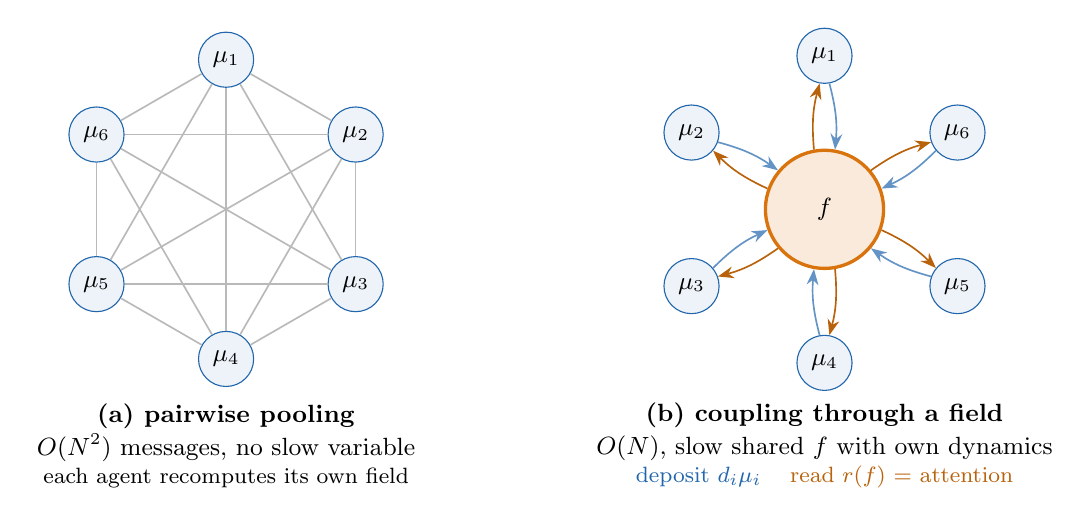
\begin{tikzpicture}[
  agent/.style={circle, draw=accent, fill=accent!8, minimum size=7mm,
                inner sep=0pt, font=\small},
  fieldn/.style={circle, draw=fieldc, very thick, fill=fieldc!15,
                 minimum size=15mm, font=\small\bfseries},
  >=Stealth
]
% ---- Panel (a): all-to-all direct pooling (a complete graph) ----
\begin{scope}
  % Nodes placed with the tikz graphs library (labelled), edges = clique.
  \graph[clockwise, radius=1.9cm, n=6, nodes={agent}]
    { 1/{$\mu_1$}, 2/{$\mu_2$}, 3/{$\mu_3$},
      4/{$\mu_4$}, 5/{$\mu_5$}, 6/{$\mu_6$} };
  \foreach \a in {1,2,3,4,5}{
    \foreach \b in {1,2,3,4,5,6}{
      \ifnum\a<\b \draw[gray!55, semithick] (\a) -- (\b);\fi}}
  \node[align=center, font=\small] at (0,-3.0)
    {\textbf{(a) pairwise pooling}\\[1pt]
     $O(N^2)$ messages, no slow variable\\[-1pt]
     \footnotesize each agent recomputes its own field};
\end{scope}
% ---- Panel (b): coupling through one shared field ----
\begin{scope}[xshift=7.6cm]
  \node[fieldn] (F) at (0,0) {$f$};
  \foreach \i/\ang in {1/90,2/150,3/210,4/270,5/330,6/30}{
    \node[agent] (A\i) at (\ang:1.95cm) {$\mu_{\i}$};
    % deposit (agent -> field), accent colour
    \draw[->, accent!70, semithick]
      (A\i) to[bend left=10] (F);
    % read / attention (field -> agent), field colour
    \draw[->, fieldc!85!black, semithick]
      (F) to[bend left=10] (A\i);
  }
  \node[align=center, font=\small] at (0,-3.0)
    {\textbf{(b) coupling through a field}\\[1pt]
     $O(N)$, slow shared $f$ with own dynamics\\[-1pt]
     \footnotesize \textcolor{accent}{deposit $d_i\mu_i$} $\;\;$
     \textcolor{fieldc!85!black}{read $r(f)$ = attention}};
\end{scope}
\end{tikzpicture}
\caption{The same coupling, two implementations. \textbf{(a)} The complete
graph $K_6$: agents pool each other's opinions directly. This is
Eq.~\eqref{eq:pairwise}; the ``field'' exists only as each agent's private,
instantaneous weighted mean. \textbf{(b)} A single shared field node $f$
mediates all coupling (Eq.~\eqref{eq:fast}--\eqref{eq:slow}): agents
\emph{deposit} into it (inward, blue) and \emph{read} from it (outward,
orange). Reading the field is the act of attending to the collective. The
field is slow ($\tau_f\!\gg\!1$) and is the only object that carries
collective state between steps.}
\label{fig:motif}
\end{figure}

\section{One motif, four substrates}
\label{sec:substrates}

The claim of this note is that Fig.~\ref{fig:motif}b is substrate-independent.
Four literatures describe the \emph{same} star-through-a-field, differing only
in what the field is made of and in the shape of the deposit/read-out
nonlinearities (Fig.~\ref{fig:fourstars}, Table~\ref{tab:substrates}).

\begin{figure}[t]
\centering
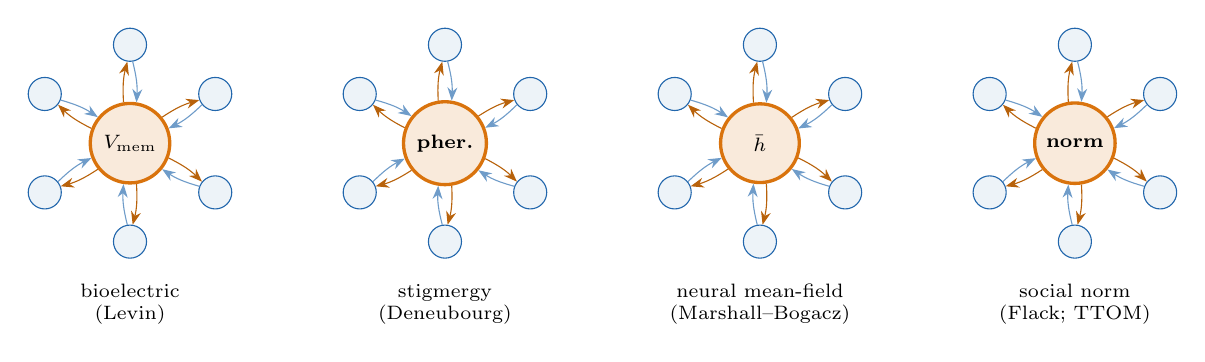
\begin{tikzpicture}[
  cell/.style={circle, draw=accent, fill=accent!8, minimum size=4.2mm, inner sep=0pt},
  fnode/.style={circle, draw=fieldc, very thick, fill=fieldc!15,
                minimum size=10mm, font=\scriptsize\bfseries, align=center},
  >=Stealth, font=\scriptsize
]
% Four sequential single-level loops (nested arrow-loops trip a pgf bug).
\node[fnode] (Fa) at (0,0) {$V_{\mathrm{mem}}$};
\foreach \ang in {30,90,150,210,270,330}{
  \node[cell] (ca-\ang) at ($(0,0)+(\ang:1.25cm)$) {};
  \draw[->, accent!65, thin] (ca-\ang) to[bend left=9] (Fa);
  \draw[->, fieldc!85!black, thin] (Fa) to[bend left=9] (ca-\ang);}
\node[align=center] at (0,-2.05) {bioelectric\\(Levin)};

\node[fnode] (Fb) at (4,0) {pher.};
\foreach \ang in {30,90,150,210,270,330}{
  \node[cell] (cb-\ang) at ($(4,0)+(\ang:1.25cm)$) {};
  \draw[->, accent!65, thin] (cb-\ang) to[bend left=9] (Fb);
  \draw[->, fieldc!85!black, thin] (Fb) to[bend left=9] (cb-\ang);}
\node[align=center] at (4,-2.05) {stigmergy\\(Deneubourg)};

\node[fnode] (Fc) at (8,0) {$\bar h$};
\foreach \ang in {30,90,150,210,270,330}{
  \node[cell] (cc-\ang) at ($(8,0)+(\ang:1.25cm)$) {};
  \draw[->, accent!65, thin] (cc-\ang) to[bend left=9] (Fc);
  \draw[->, fieldc!85!black, thin] (Fc) to[bend left=9] (cc-\ang);}
\node[align=center] at (8,-2.05) {neural mean-field\\(Marshall--Bogacz)};

\node[fnode] (Fd) at (12,0) {norm};
\foreach \ang in {30,90,150,210,270,330}{
  \node[cell] (cd-\ang) at ($(12,0)+(\ang:1.25cm)$) {};
  \draw[->, accent!65, thin] (cd-\ang) to[bend left=9] (Fd);
  \draw[->, fieldc!85!black, thin] (Fd) to[bend left=9] (cd-\ang);}
\node[align=center] at (12,-2.05) {social norm\\(Flack; TTOM)};
\end{tikzpicture}
\caption{The mediating field across scales. In every case a population of
units couples \emph{only} through a slow shared field they both write
($\rightarrow$ in) and sense ($\rightarrow$ out): transmembrane voltage
$V_{\mathrm{mem}}$ patterning tissue; the pheromone concentration on a trail;
the mean activity $\bar h$ of a competing neural population; the consensus
``power structure''/norm a community references. The topology is identical
to Fig.~\ref{fig:motif}b.}
\label{fig:fourstars}
\end{figure}

\begin{table}[t]
\centering
\renewcommand{\arraystretch}{1.25}
\begin{tabular}{@{}p{2.5cm} p{2.4cm} p{2.6cm} p{2.6cm} p{2.5cm}@{}}
\toprule
 & \textbf{Bioelectric} & \textbf{Stigmergic} & \textbf{Neural} & \textbf{Social} \\
\midrule
Field $f$        & transmembrane voltage $V_{\mathrm{mem}}$ & pheromone conc.\ & pop.\ mean activity $\bar h$ & shared norm / power \\
Deposit $g$      & ion-channel flux & trail laying & spiking & public claim, citation \\
Evaporate $1/\tau_f$ & gap-junction leak & chemical decay & adaptation & forgetting, turnover \\
Read = attention & sense $V_{\mathrm{mem}}$ gradient & follow gradient & recurrent input & defer to norm \\
Nonlinearity     & voltage-gated channels & comparative trail choice & cross-inhibition & comparative status \\
Bistable?        & pattern memory & symmetry-broken trail & DDM decision & paradigm lock-in \\
Reference        & \cite{Levin2014,PezzuloLevin2016} & \cite{Deneubourg1990} & \cite{MarshallBogacz2009} & \cite{Flack2017,TTOM2020} \\
\bottomrule
\end{tabular}
\caption{One motif, four substrates. Rows are the components of
Eqs.~\eqref{eq:fast}--\eqref{eq:slow}; columns are the physical realisations.
The shared structure is the point: a slow field, written and read, with the
listening nonlinearity living in the deposit/read-out.}
\label{tab:substrates}
\end{table}

\section{Reading the field is attention}
\label{sec:attention}

In Eq.~\eqref{eq:fast} the gain $\pi_i$ on the read-out term is precisely the
\emph{precision} an agent assigns to the collective field --- how much it
lets the consensus move its belief. This is the social Hierarchical
Gaussian Filter reading of trust \cite{Diaconescu2017}: trust is not a row
of a mixing matrix but the learned reliability (precision) of a channel.
Two limits make the unification concrete.
\begin{itemize}
\item \textbf{Uniform precision} ($\pi_i$ equal, $r(f)=f=$ mean): linear
  averaging, DeGroot, consensus. The honeybee's proportional response.
\item \textbf{Peaked precision} (one source dominates): the read-out
  collapses onto a single voice --- ``listen to the most knowledgeable.''
  No separate mechanism; the same field-read at a different precision.
\end{itemize}
The community's \emph{norm} is then the prior on these precisions --- a
``regime of expectations'' \cite{TTOM2020} specifying how members should
weight the field. And because the field is externalised (Table~\ref{tab:substrates}),
that prior need not be estimated by any central node: it is the standing
state of $f$ itself, read by all. This is the stigmergic resolution of the
decentralisation problem --- the norm lives in the trail, not in a head.

\section{The nonlinearity decides the phase}
\label{sec:phase}

With the field explicit, the question ``linear or nonlinear pooling?''
becomes sharp and is answered by a measured natural experiment in the
foraging literature (Fig.~\ref{fig:response}). If the per-agent response to
the field is \emph{proportional} (honeybee), the symmetric consensus state
is the only attractor. If it is \emph{comparative and amplifying}
(ant; Deneubourg's $q^n/(q^n+(1-q)^n)$), the symmetric state goes unstable
and the field breaks symmetry into one of two locked states --- bistability,
i.e.\ paradigm lock-in.

\begin{figure}[t]
\centering
\begin{minipage}{0.48\textwidth}
\centering
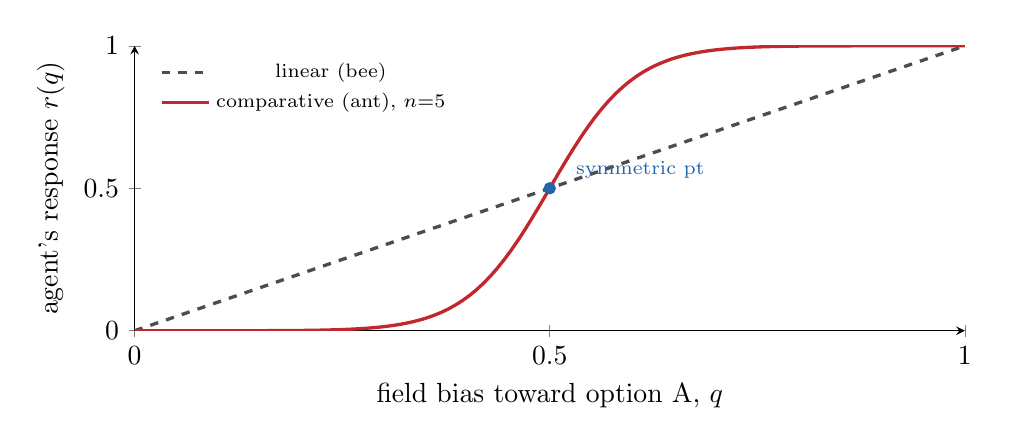
\begin{tikzpicture}
\begin{axis}[
  width=\textwidth, height=5.2cm,
  xlabel={field bias toward option A, $q$},
  ylabel={agent's response $r(q)$},
  domain=0:1, samples=120,
  xmin=0, xmax=1, ymin=0, ymax=1,
  xtick={0,0.5,1}, ytick={0,0.5,1},
  legend style={at={(0.02,0.98)}, anchor=north west, font=\scriptsize, draw=none},
  axis lines=left, every axis plot/.append style={very thick}
]
\addplot[neutralg, dashed] {x};
\addlegendentry{linear (bee)}
\addplot[unstable] {x^5/(x^5+(1-x)^5)};
\addlegendentry{comparative (ant), $n{=}5$}
\addplot[only marks, mark=*, mark size=1.6pt, accent]
  coordinates {(0.5,0.5)};
\node[font=\scriptsize, accent, anchor=south west] at (axis cs:0.52,0.5)
  {symmetric pt};
\end{axis}
\end{tikzpicture}
\\[2pt]{\footnotesize (a) listening response to the field}
\end{minipage}\hfill
\begin{minipage}{0.48\textwidth}
\centering
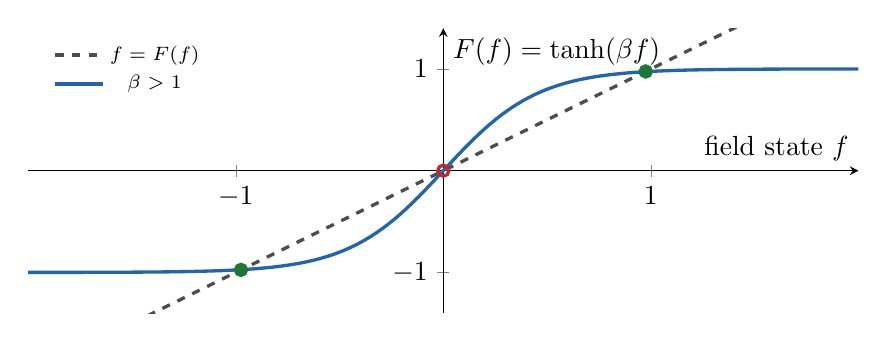
\begin{tikzpicture}
\begin{axis}[
  width=\textwidth, height=5.2cm,
  xlabel={field state $f$}, ylabel={$F(f)=\tanh(\beta f)$},
  domain=-2:2, samples=120,
  xmin=-2, xmax=2, ymin=-1.4, ymax=1.4,
  xtick={-1,0,1}, ytick={-1,0,1},
  axis lines=middle, every axis plot/.append style={very thick},
  legend style={at={(0.02,0.98)}, anchor=north west, font=\scriptsize, draw=none}
]
\addplot[neutralg, dashed] {x};
\addlegendentry{$f=F(f)$}
\addplot[accent] {tanh(2.2*x)};
\addlegendentry{$\beta>1$}
\addplot[only marks, mark=*, mark size=2pt, stable]
  coordinates {(0.975,0.975) (-0.975,-0.975)};
\addplot[only marks, mark=o, mark size=2pt, unstable]
  coordinates {(0,0)};
\end{axis}
\end{tikzpicture}
\\[2pt]{\footnotesize (b) self-consistency $f=F(f)$}
\end{minipage}
\caption{Where bistability comes from. \textbf{(a)} The per-agent read-out
$r(q)$. Bee = linear/proportional (grey dashed) $\Rightarrow$ slope $1$ at
the symmetric point $q=\tfrac12$, marginal. Ant = comparative amplification
(red) $\Rightarrow$ slope $>1$ at $q=\tfrac12$, so the symmetric state is
unstable. The \emph{degree of nonlinearity of the listening response} is the
bifurcation parameter \cite{Deneubourg1990}. \textbf{(b)} The same statement
as a mean-field self-consistency condition $f=F(f)$ (Flack's circular
causality: the field is computed from the population it then steers). When
the slope $\beta$ of the deposit$\circ$read-out loop exceeds $1$, the
fixed point $f=0$ (open red, unstable) loses stability and two stable
fixed points appear (filled green) --- the fold that makes a paradigm
self-sustaining \cite{Flack2017,BizyaevaFranciLeonard2023}.}
\label{fig:response}
\end{figure}

\begin{proposition}[Field-mediated bistability]
Let agents relax quickly to the field ($\alpha,\beta$ fast) and let the field
obey $\tau_f\dot f = -f + F(f)$ with $F$ the composition of deposit and
read-out over the (fast-equilibrated) population. If $F'(f^\ast)>1$ at the
symmetric fixed point, that point is unstable and, for bounded sigmoidal
$F$, two stable fixed points exist. Bistability is thus a property of the
\emph{slow field's} self-consistency loop, not of any single agent's update.
\end{proposition}

\noindent This is the honest location of the phenomenon. Linear pooling
(Fig.~\ref{fig:response}a, grey) keeps $F'\le 1$ and cannot fold; a
comparative/cross-inhibitory read-out pushes $F'>1$ and can. It also says
\emph{why} an over-informative environment defeats the effect: a large
$\alpha$ pull toward $\theta^\ast$ flattens the effective $F$, and the
relevant competition is $\,F' \;\text{vs}\; 1\,$ once the environment is
folded in --- a clean, interpretable line rather than a magic coefficient.

\section{Consequences for the active-inference rebuild}
\label{sec:rebuild}

\begin{enumerate}
\item \textbf{Add a field, not more edges.} Represent $f$ explicitly as a
  slow shared state (a stigmergic ``trail'' over paradigms). In the
  categorical \texttt{pymdp} rebuild this is a shared object agents observe
  as a modality and deposit into --- $O(N)$, and it carries the collective
  memory between steps.
\item \textbf{Put the nonlinearity in the read-out, derived not designed.}
  Use comparative/cross-inhibitory reading (the optimal-decision motif of
  \cite{MarshallBogacz2009}) so $F'>1$ is reachable. Avoid a hand-tuned
  $\tanh$ on the coupling; derive the inhibition from the decision the agent
  is actually making.
\item \textbf{Trust = read-out precision $\pi_i$, with the norm as its prior.}
  This makes trust load-bearing (it sets $F'$, hence the phase) rather than
  decorative, and frames the community norm as the standing field state.
\item \textbf{Test the fold, not the trajectory.} The pivotal experiment is
  whether $F'>1$ is attainable against the environment's $\alpha$ ---
  measure the self-consistency curve (Fig.~\ref{fig:response}b) directly
  rather than hunting for hysteresis in time series.
\end{enumerate}

\begin{thebibliography}{9}
\bibitem{Levin2014} M.~Levin. Endogenous bioelectrical networks store
non-genetic patterning information during development and regeneration.
\emph{J.\ Physiol.}, 592(11):2295--2305, 2014.
\bibitem{PezzuloLevin2016} G.~Pezzulo and M.~Levin. Top-down models in
biology: explanation and control of complex living systems above the
molecular level. \emph{J.\ R.\ Soc.\ Interface}, 13(124):20160555, 2016.
\bibitem{Deneubourg1990} J.-L.~Deneubourg et al. The self-organizing
exploratory pattern of the Argentine ant. \emph{J.\ Insect Behavior},
3:159--168, 1990.
\bibitem{MarshallBogacz2009} J.~A.~R.~Marshall, R.~Bogacz, et al. On optimal
decision-making in brains and social insect colonies. \emph{J.\ R.\ Soc.\
Interface}, 6(40):1065--1074, 2009.
\bibitem{Flack2017} J.~C.~Flack. Coarse-graining as a downward causation
mechanism. \emph{Phil.\ Trans.\ R.\ Soc.\ A}, 375:20160338, 2017.
\bibitem{TTOM2020} S.~P.~L.~Veissi\`ere, A.~Constant, M.~J.~D.~Ramstead,
K.~J.~Friston, L.~J.~Kirmayer. Thinking through other minds: A variational
approach to cognition and culture. \emph{Behavioral and Brain Sciences},
43:e90, 2020.
\bibitem{Diaconescu2017} A.~O.~Diaconescu et al. Hierarchical prediction
errors in midbrain and septum during social learning. \emph{Soc.\ Cogn.\
Affect.\ Neurosci.}, 12(4):618--634, 2017.
\bibitem{BizyaevaFranciLeonard2023} A.~Bizyaeva, A.~Franci, N.~E.~Leonard.
Nonlinear opinion dynamics with tunable sensitivity. \emph{IEEE Trans.\
Automatic Control}, 68(3):1415--1430, 2023.
\end{thebibliography}

\end{document}
